\documentclass[a4paper,ngerman,14pt,landscape]{article}
\usepackage[utf8]{inputenc}
\usepackage[ngerman]{babel}
\usepackage{graphicx}
\usepackage{setspace}
\usepackage{geometry}
\geometry{tmargin=3cm,bmargin=2cm,lmargin=3cm,rmargin=3cm}

\pagestyle{empty}

\renewcommand*{\familydefault}{\sfdefault}

\setlength{\unitlength}{1cm}

\begin{document}

\begin{picture}(0,0)
  \put(20,-0){%
    
\includegraphics[scale=0.15]{logo-uni}
  }
  \put(19,-16){%
    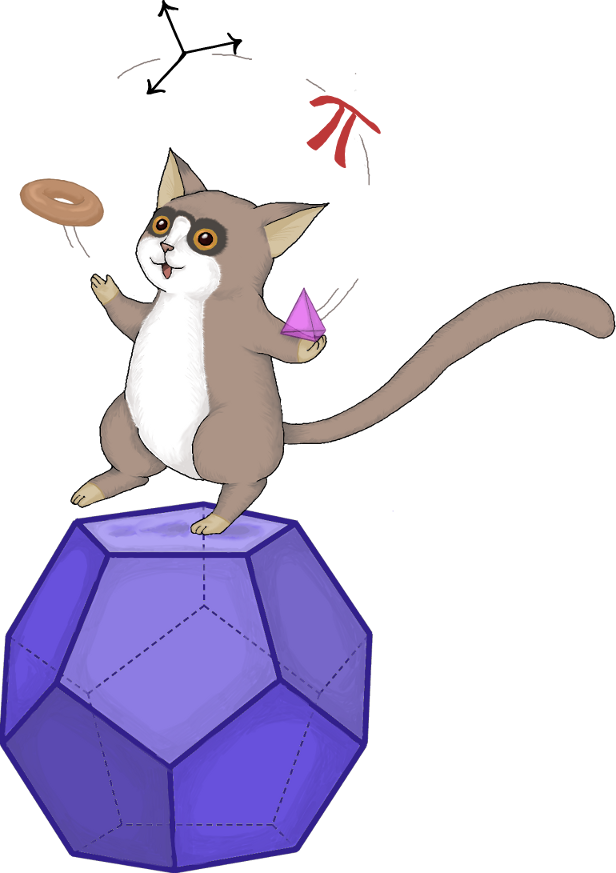
\includegraphics[scale=0.18]{illustrationen/cover}
  }
\end{picture}
\vspace{-7em}

\doublespacing

\Huge

\begin{center}
  \textbf{Matheschülerzirkel Augsburg}
\end{center}
\vspace{0.2em}

\Huge

\begin{tabbing}
  10:00 Uhr:\quad \= \kill
  10:00 Uhr: \> Begrüßung durch Prof. Dr. Marco Hien \\
  10:05 Uhr: \> Allgemeine Informationen \\[0.5em]
  10:20 Uhr: \> Vortrag von Prof. Dr. Jost-Hinrich Eschenburg \\
  \> \emph{Was sind eigentlich die Zahlen?} \\[0.5em]
  11:00 Uhr: \> Pause mit Getränken und Butterbrezen, \\
  \> Möglichkeit für Fragen \\[0.5em]
  11:20 Uhr: \> Einteilung der Gruppen, Terminfindung \\
  danach: \> Ende der Veranstaltung
\end{tabbing}

\end{document}
